\section{Simulation Analysis}
\label{section:sim}
 
In this section, the several steps taken using ngspice in order to conduct the simulation of the band pass filter using an OP-AMP, as requested, will be described. The main focus of the simulation was to determine and optimize the values of the gain, the central frequency and the output and input impedances. The quality and overall figure of merit will then be analysed.
The group proceded as follows:

\begin{enumerate}
\item Design of the circuit, having as a starting point the circuit presented in section \ref{introduction}

  
\item  In the frequency domain, measure of the output voltage gain, using the function .meas as well as the lower and upper cut off frequencies and the central frequency.


\begin{table}[ht]
  \centering
  \begin{tabular}{|l|r|}
    \hline    
   Gain& 34.0105\\ \hline
Central Frequency& 794.328\\ \hline
Gain deviation&49.8206\\ \hline
Central frequency deviation&205.672\\ \hline

    \end{tabular}
  \caption{Results for ngspice}
    \label{tab:results}
\end{table}


Then, the response of the circuit in dB and the phase were computed. The gain was also determined. In fact, the main goal of the assignement was to design a band pass filter. This means that this filter should cut both low an very high frequencies. THis is precisely what is shown in figure \ref{fig:gain}




\begin{figure}[ht]
\centering
\begin{subfigure}{.5\textwidth}
  \centering
  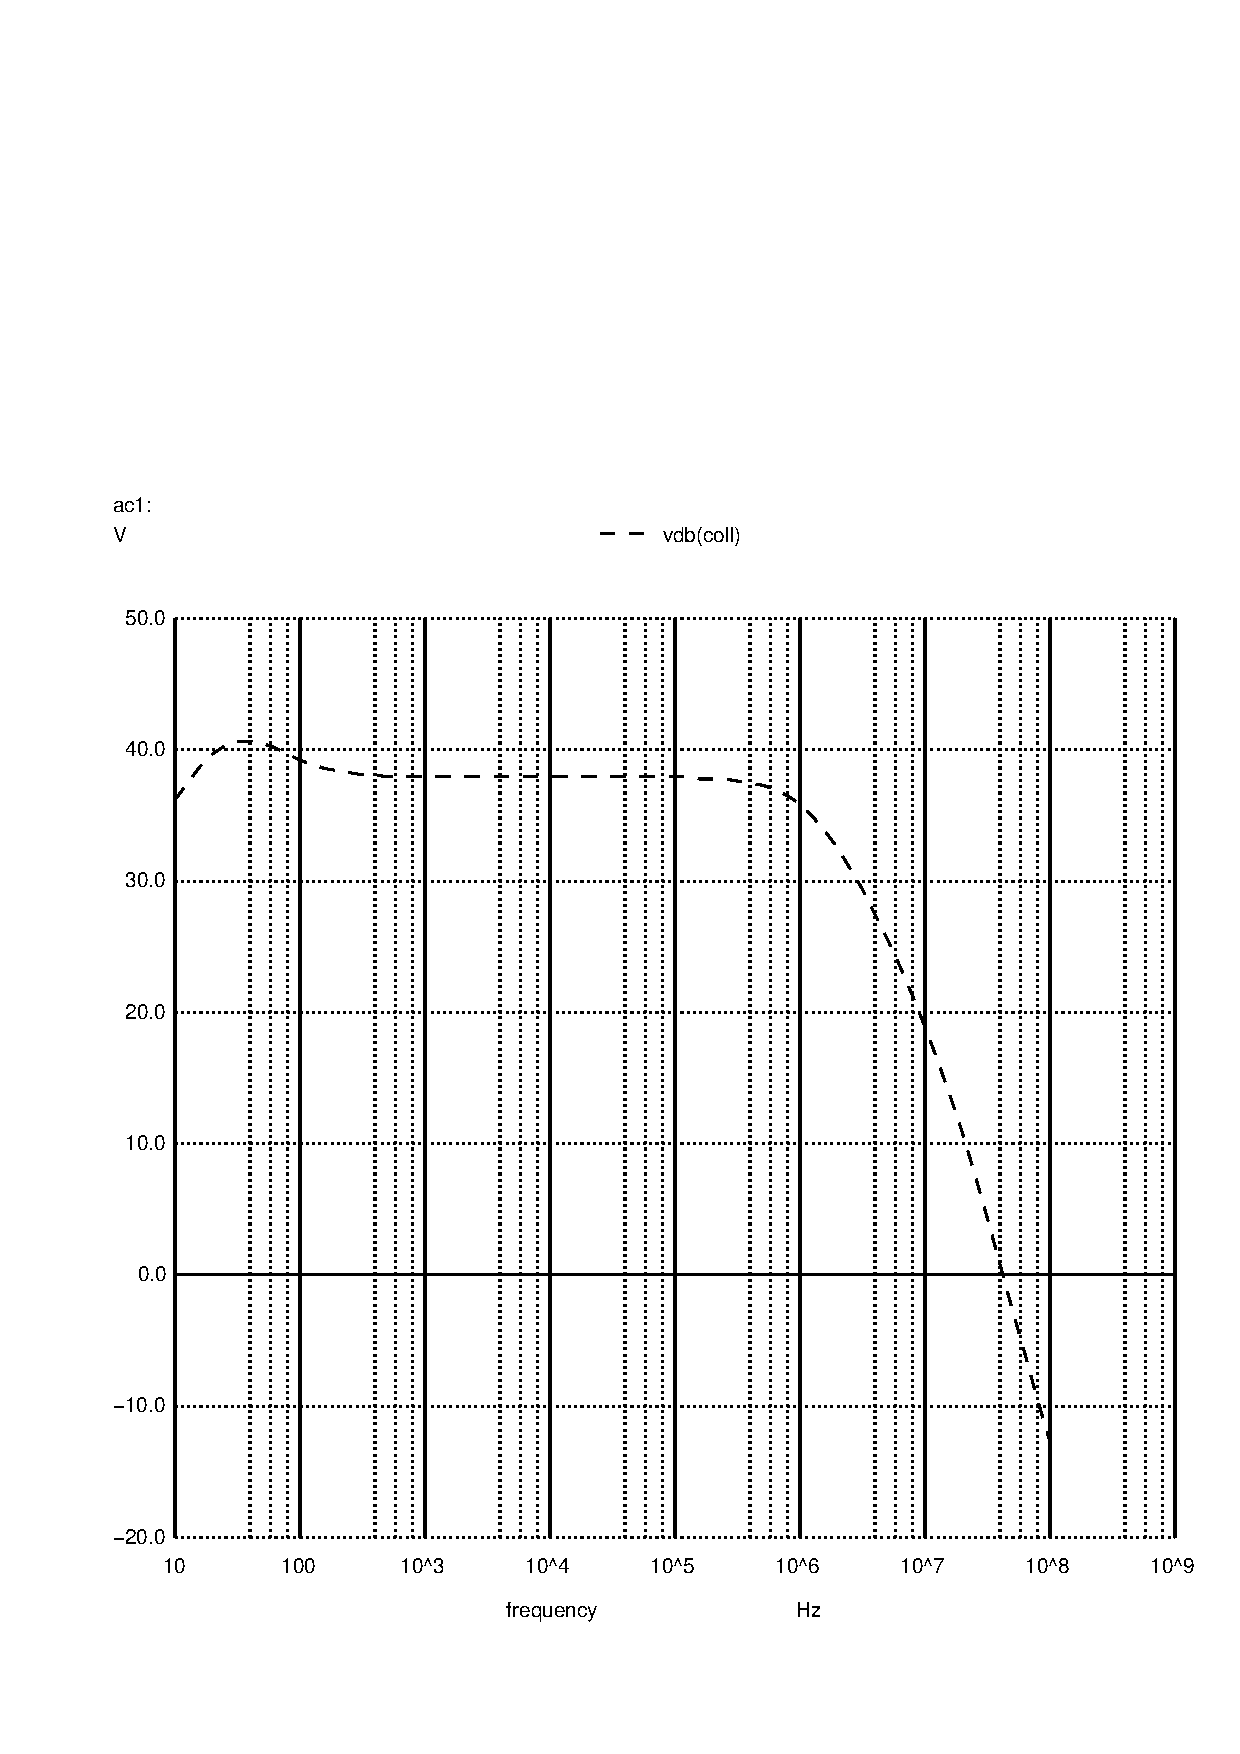
\includegraphics[width=.45\linewidth]{vo1f.pdf}
  \caption{Output Voltage in dB}
  \label{fig:sim5}
\end{subfigure}%
\begin{subfigure}{.5\textwidth}
  \centering
  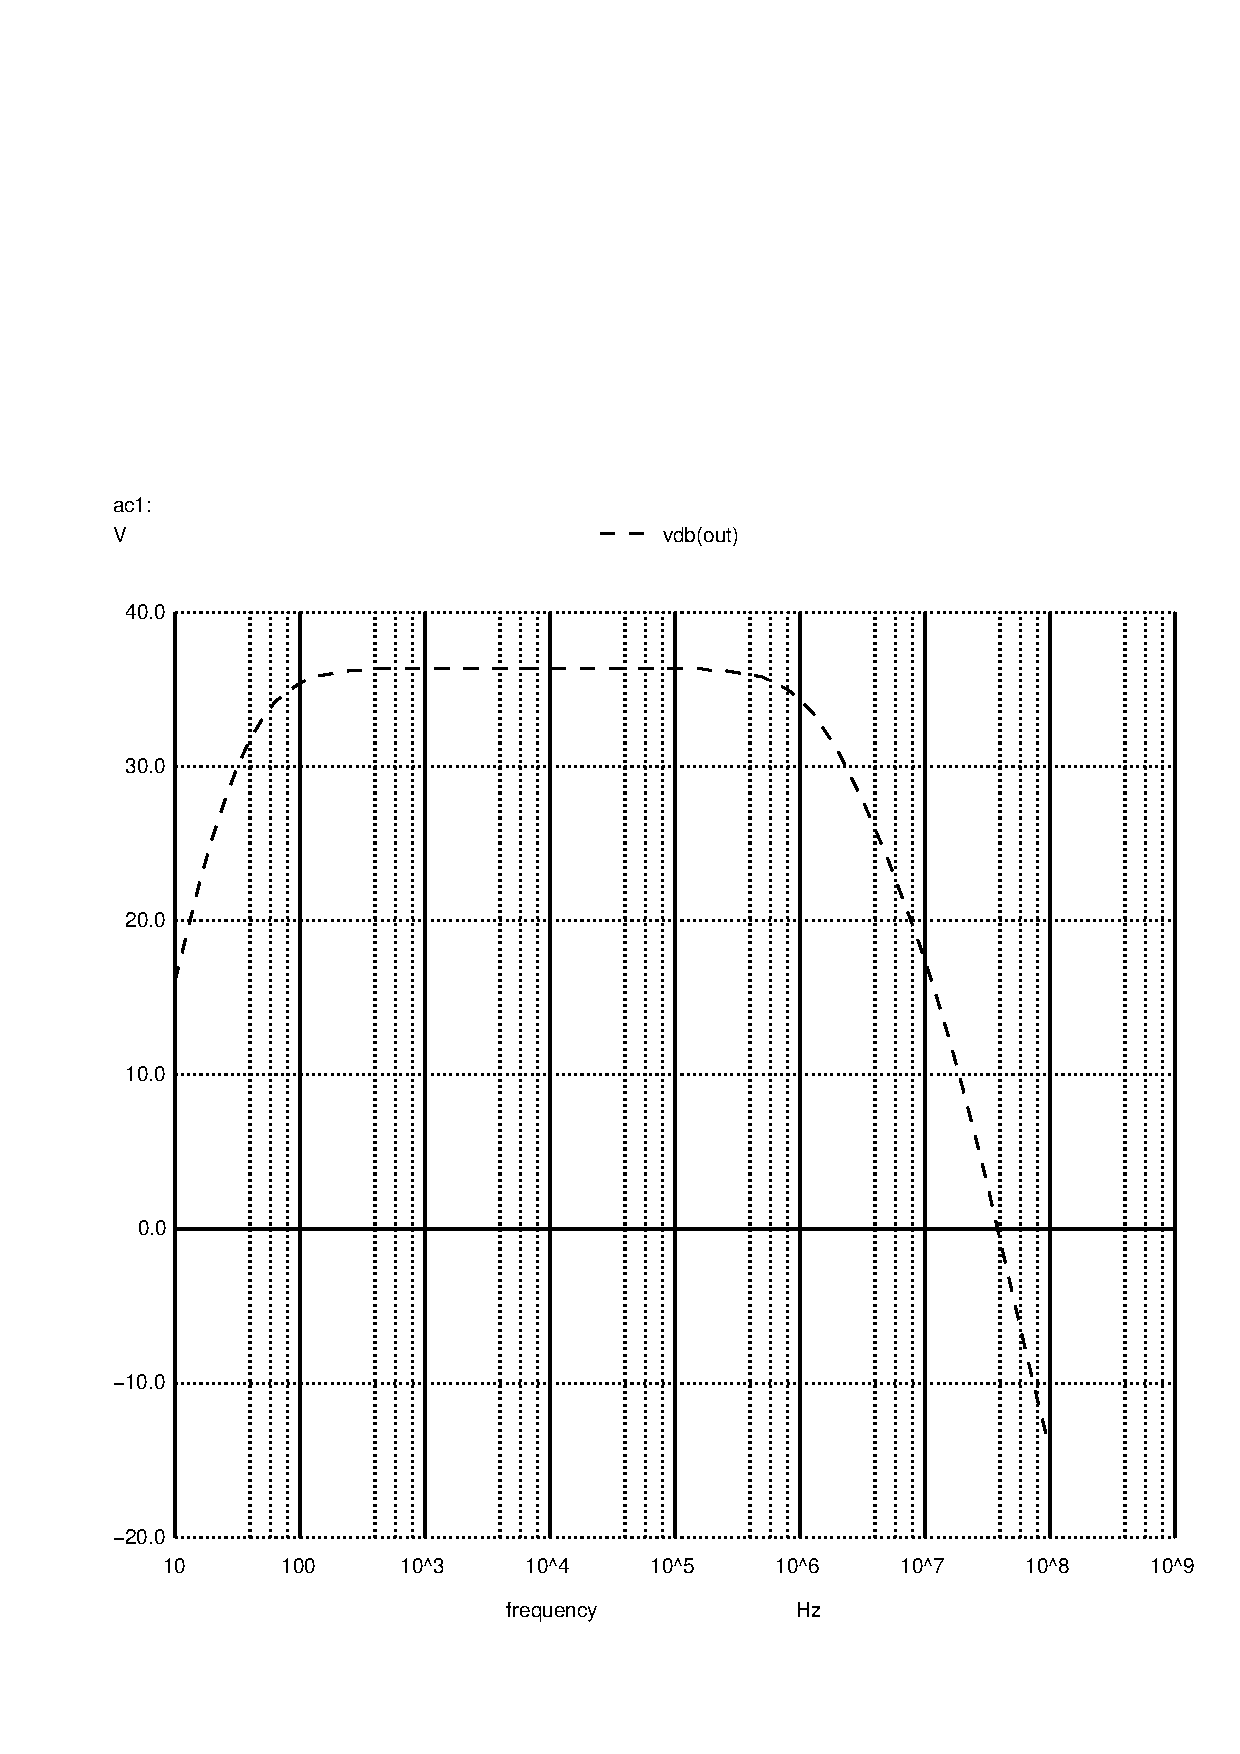
\includegraphics[width=.45\linewidth]{vo2f.pdf}
  \caption{Output voltage (phase)}
  \label{fig:sim6}
  \end{subfigure}
  \begin{subfigure}{.5\textwidth}
  \centering
  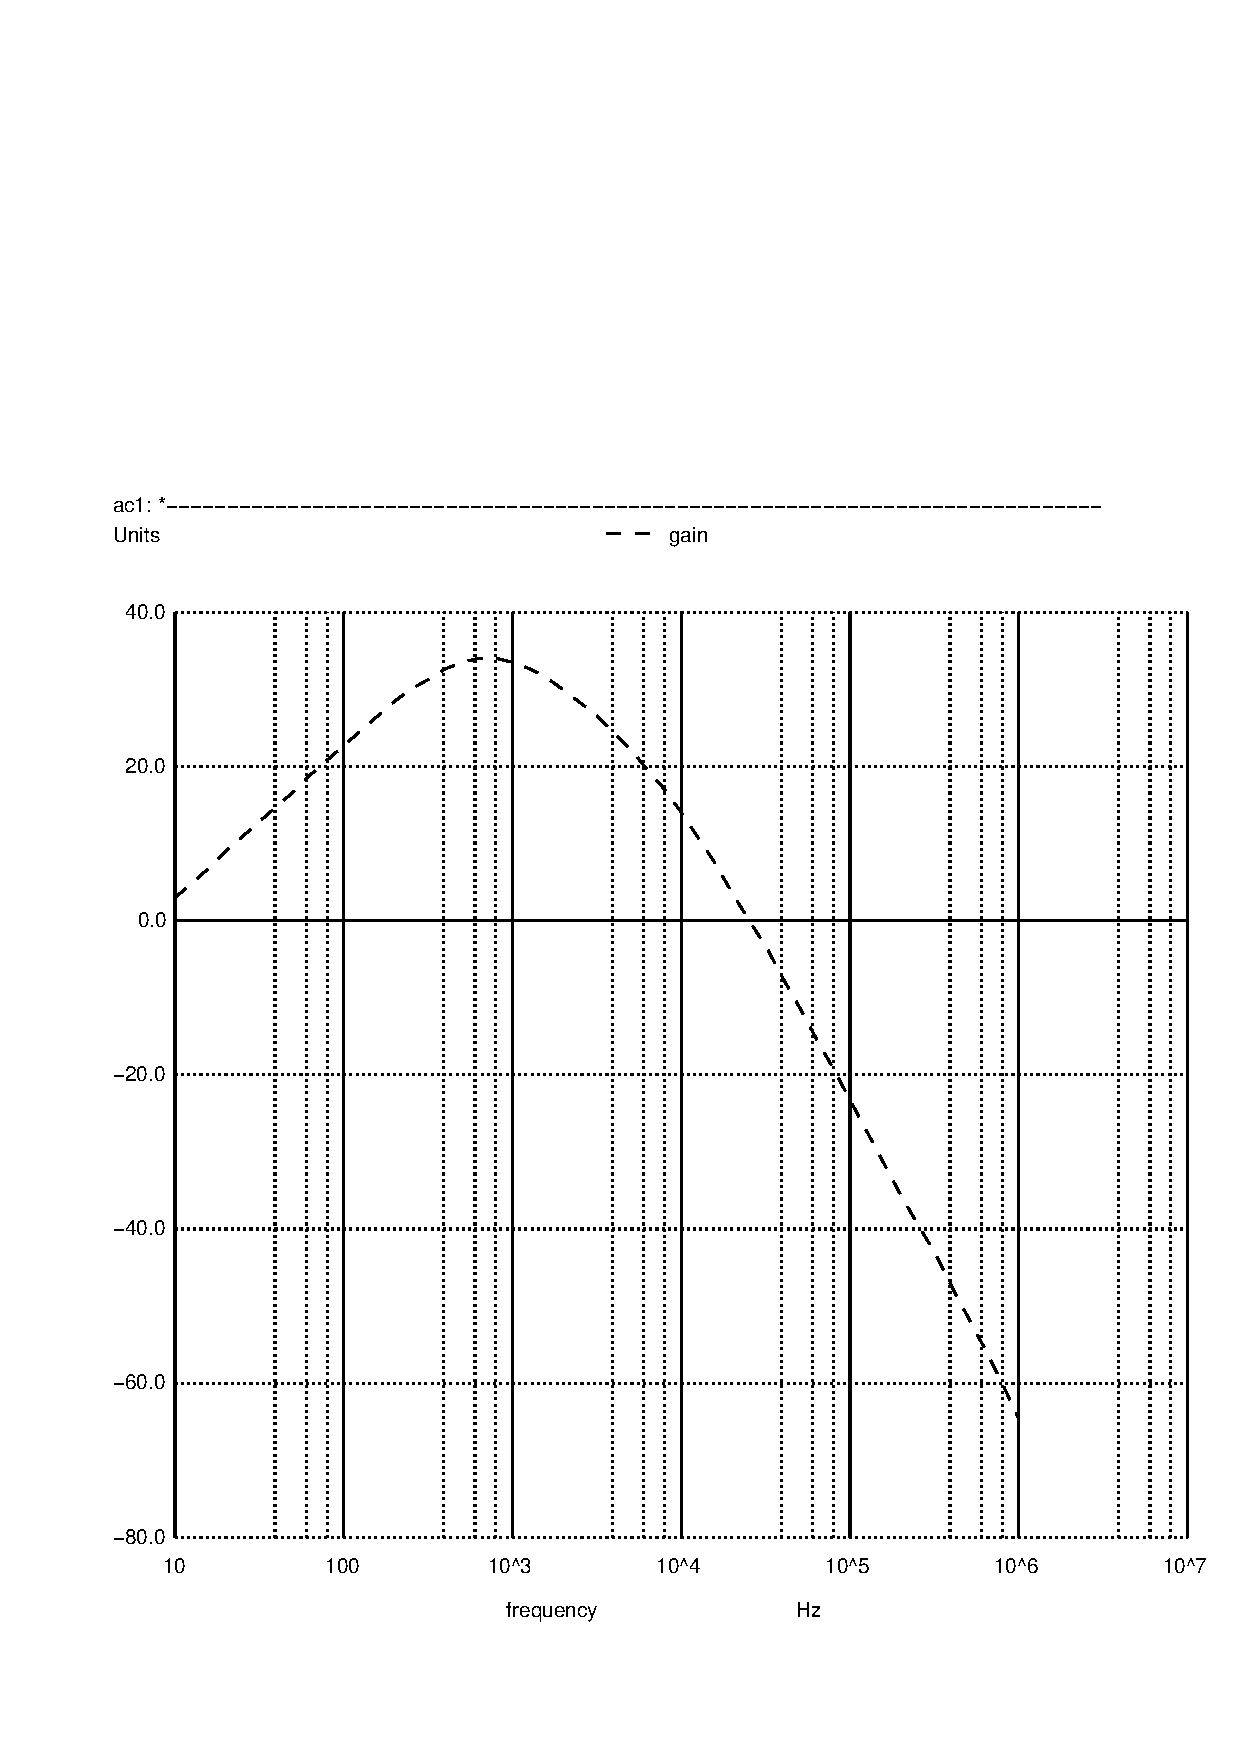
\includegraphics[width=.45\linewidth]{gain.pdf}
  \caption{Gain}
  \label{fig:sim6}

\end{subfigure}
\end{figure}



\item Determination of the input impedance, seen from the input voltage source.

\begin{table}[h]
  \centering
  \begin{tabular}{|l|r|}
    \hline    
   Zin & 999.002 + -7.3282 j\\ \hline

   \end{tabular}
  \caption{Input impedance in Ohm}
    \label{tab:ZI}
\end{table}

\par The result obtained for the input impedance, considering the value in Ohm, is high. This is benefitial for the gain, because the voltage in the node In 2 must be as similiar to Vin as possible. Using a voltage divider, the only way to achieve this was to have a very high resistance value.

\item Determination of the output impedance, using a different set up, seen from the load resistance. 

\begin{table}[h]
  \centering
  \begin{tabular}{|l|r|}
    \hline    
   Zo & 0.0522978 + -7.23396 j\\ \hline

   \end{tabular}
  \caption{Output impedance in Ohm}
  
  \label{tab:ZO}
\end{table}


Conserning the output impedance, an opposite deduction to the one made for the output impedance is mandoratory. Considering a voltage divider, the output impedance must be as low as possible, in order to the output voltage to be as high as possible. Having said that, an analysing tables \ref{tab:ZI} \ref{tab:ZO}, the difference needed between the two is confirmed. 

\item Compute of the cost and figure of merit
\par To finally understand the efficency of the amplifier, the cost and figure of merit were calculated

\begin{table}[ht]
  \centering
  \begin{tabular}{|l|r|}
    \hline    
   Cost & 1225.6\\ \hline
merit & 716.238\\ \hline

   \end{tabular}
  \caption{Cost and Figure of merit}
  \label{tab:cost}
\end{table}

Analysing table \ref{tab:cost}, the results obtained may be considered satisfying.


\end{enumerate}



